\section{Model}
\begin{figure*}[ht]
    \centering
    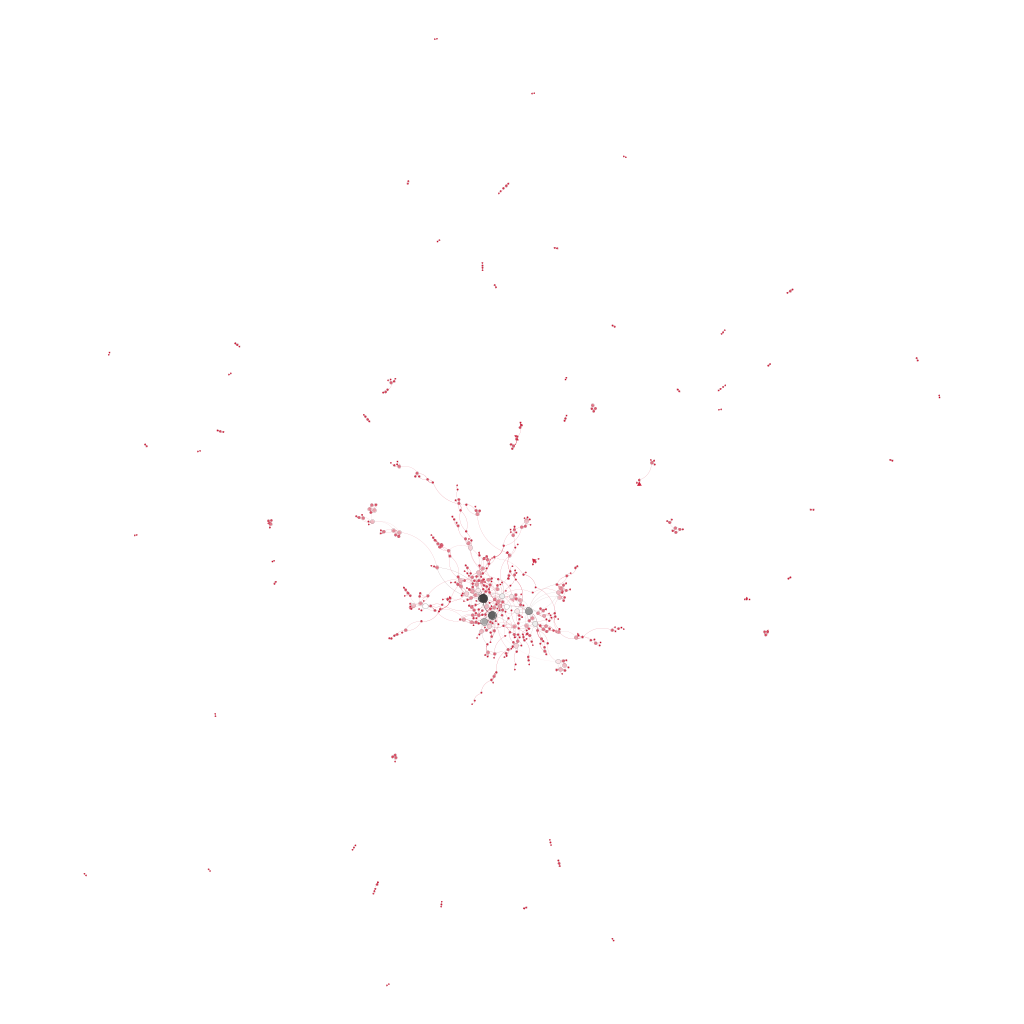
\includegraphics[width=0.3\linewidth]{figures/Calls_network.png}
    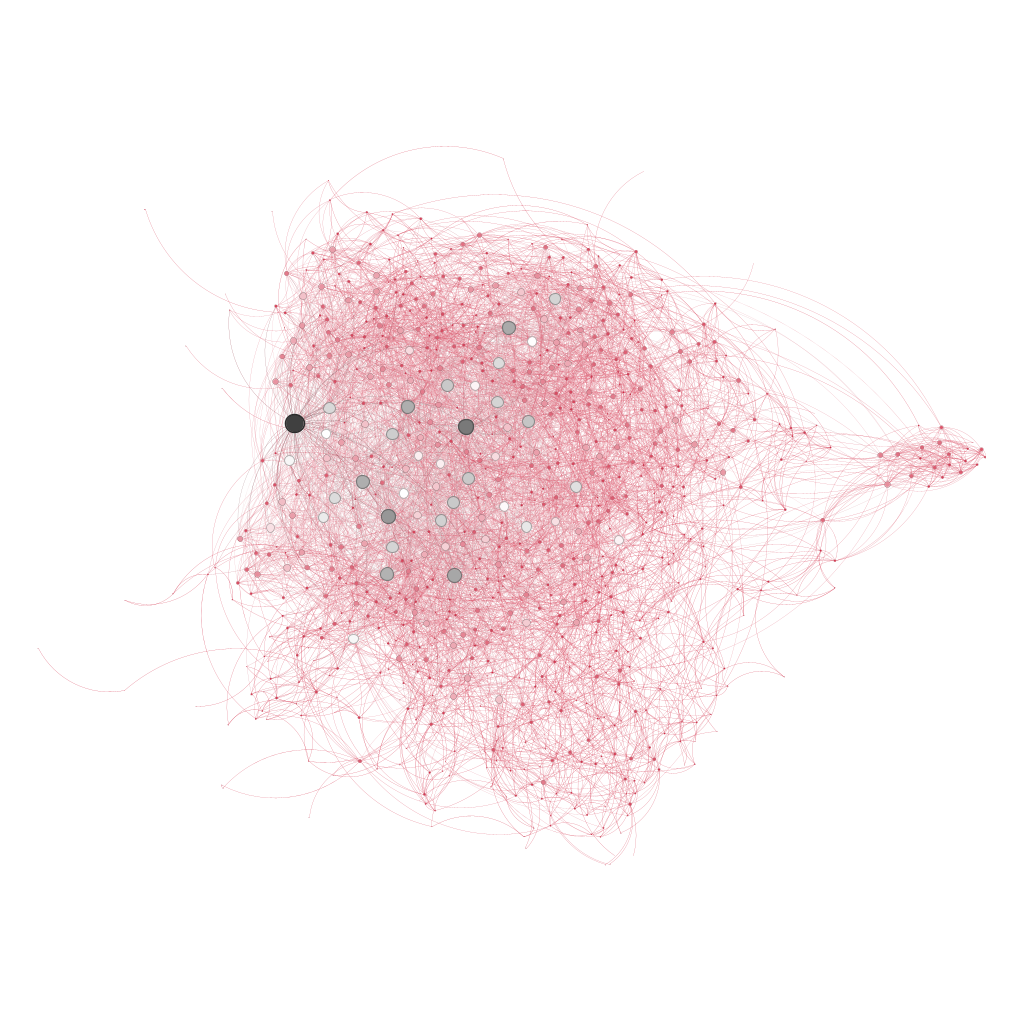
\includegraphics[width=0.3\linewidth]{figures/FB_network.png}
    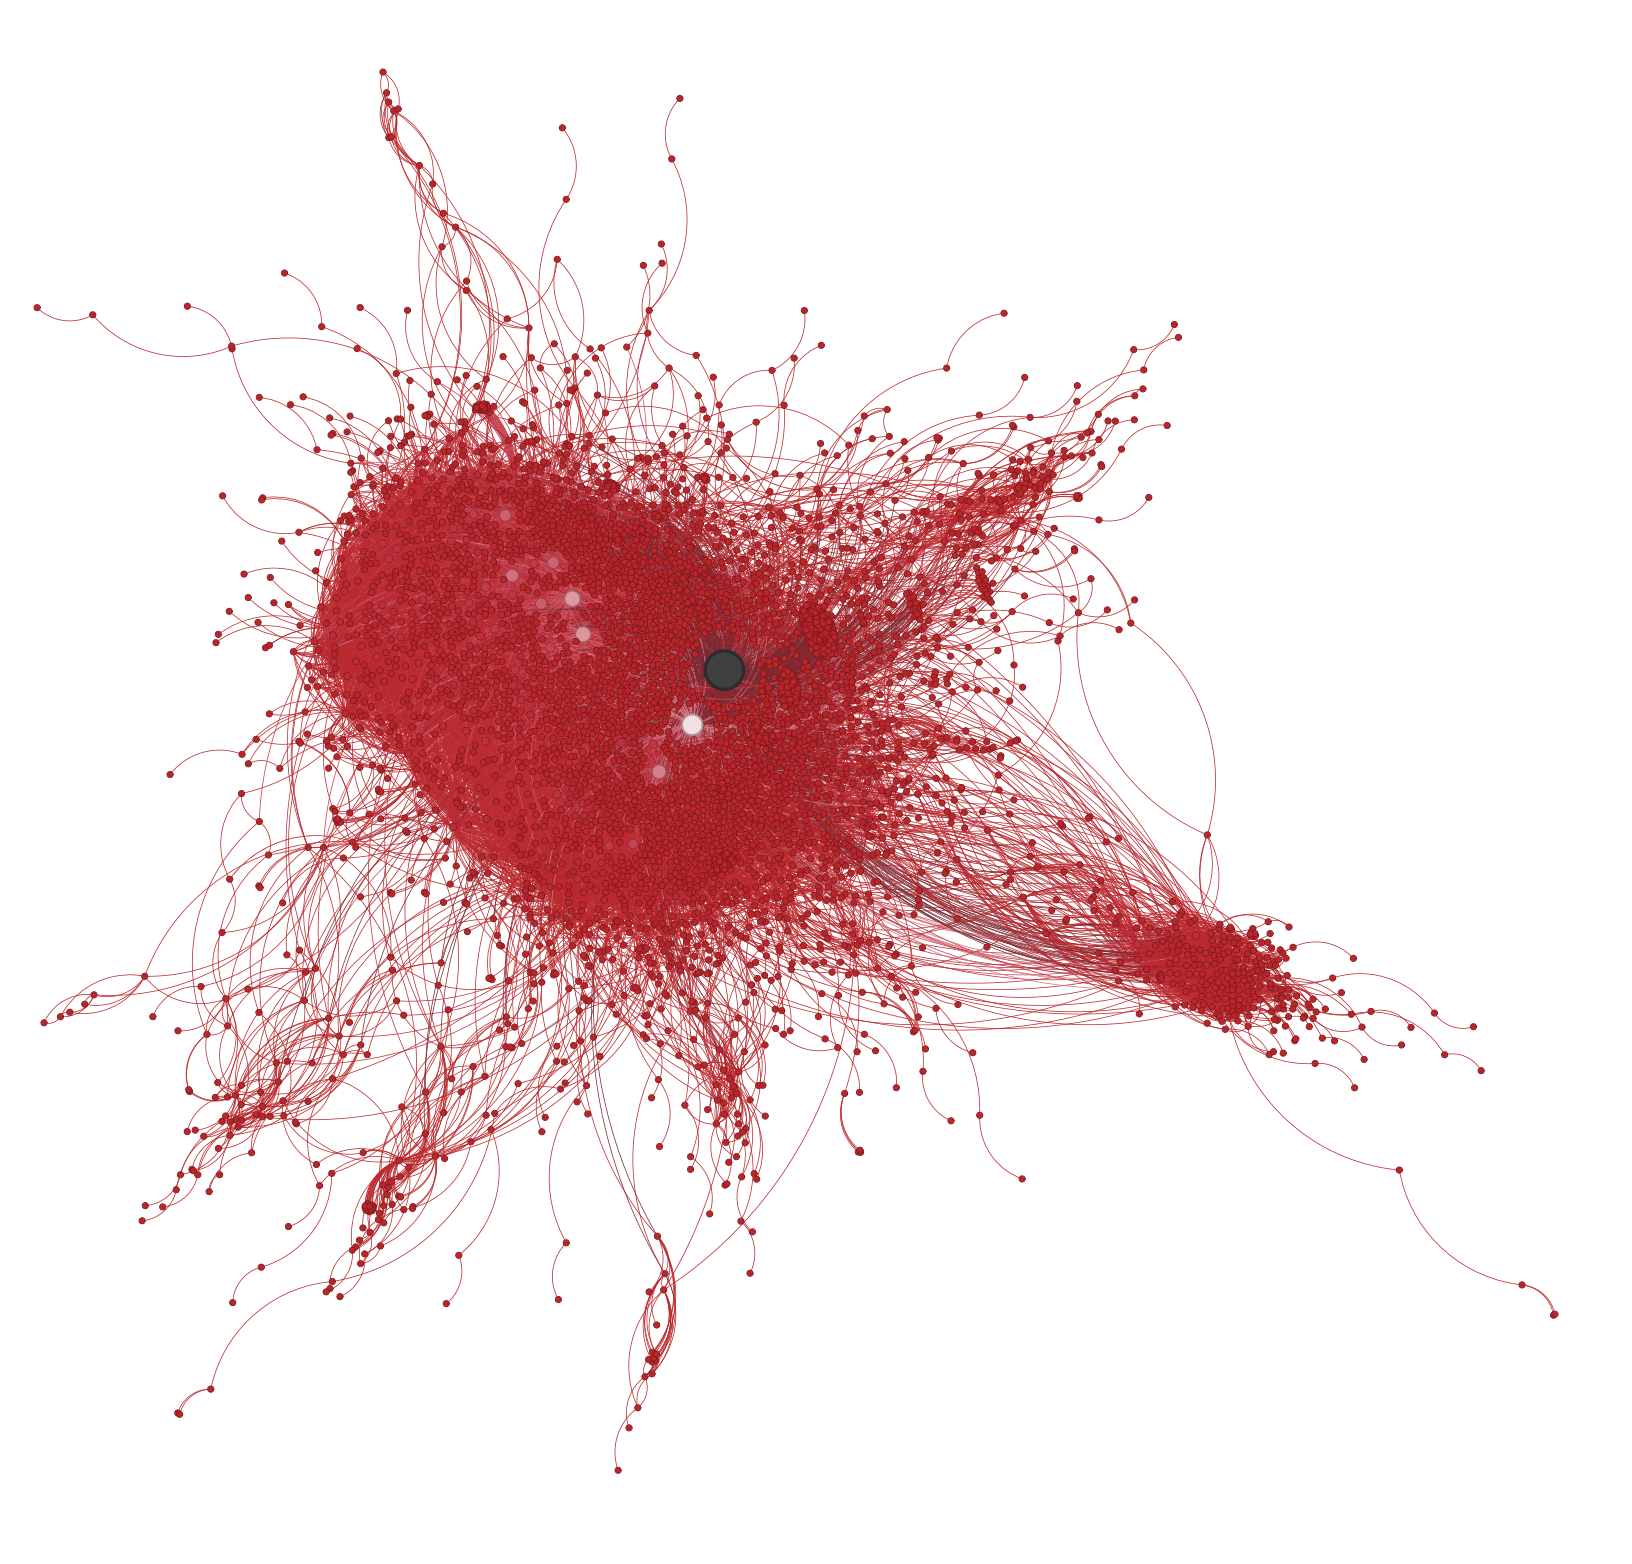
\includegraphics[width=0.3\linewidth]{figures/ff.png}
    \caption{Figure example}
    \label{fig:enter-label}
\end{figure*}


The first network we looked at was the Facebook dataset (SNAP). This network consists of anonymized ego-networks extracted from Facebook, where each node represents a user and edges represent friendship links. Using this as our base, we assigned each node’s initial strategy with a Bernoulli (0.5) distribution, giving an equal chance between cooperation and defection. Then, after every game iteration playing Prisoner’s Dilemma, there is an update strategy where each node will look at all its neighbors and will adopt the more successful strategy. 
The next network we looked at was the Epinions social network dataset (SNAP), a directed “who-trusts-whom” graph from the Epinions.com review site, where each edge indicates that one user has marked another as trusted or not trusted. 
